\documentclass[11pt]{report}
\usepackage[utf8]{inputenc} 
\usepackage[backend=bibtex, maxnames=5]{biblatex}
\usepackage[T1]{fontenc}
\usepackage[english]{babel}  
\usepackage[pdftex]{graphicx}
\usepackage[titles]{tocloft}
\usepackage{amsthm}
\usepackage{amsmath}
\usepackage{amssymb}
\usepackage{mathrsfs} 
\usepackage{enumitem}
\usepackage[babel=true]{csquotes}
\usepackage{wrapfig}
\usepackage{soul}
\usepackage[right=1.25in,left=1.25in,top=1.in,bottom=1.in]{geometry}  %% right=0.75in,left=0.75in,top=0.75in,bottom=0.75in
\usepackage{etoolbox}
\usepackage[toc,page]{appendix}
\usepackage{caption}
%\usepackage{captionof}
\usepackage{subfig}
\usepackage{pdfpages}
\usepackage{titlesec}
\usepackage{fancyhdr}
%\usepackage[nottoc]{tocbibind}
\usepackage{fancyhdr,lastpage}
\usepackage{array}
\usepackage{eurosym}
\usepackage[hidelinks]{hyperref}
\usepackage{todonotes}
\usepackage{lipsum}
\usepackage{svg}

\bibliography{PDM_references.bib}

\graphicspath{{../figures/}}
\titleformat{\chapter}[hang]{\normalfont\huge\bfseries}{\thechapter.}{20pt}{\huge}

\title{Spherical Convolutional Neural Networks}
\author{Frédérick Matthieu Gusset}

\makeatletter
\let\thetitle\@title
\let\theauthor\@author
\makeatother

\DeclareMathSizes{10}{11}{8}{8}   % Pour un texte de taille 10 
\titlespacing*{\chapter} {0pt}{15pt}{15pt}
\makeatletter
\patchcmd{\printbibliography}{%
 \chapter*{\bibname}\@mkboth{\MakeUppercase\bibname}{\MakeUppercase\bibname}}{%
 \chapter{References}}{}{}
\makeatother

\renewcommand{\headrulewidth}{0pt}
\renewcommand{\footrulewidth}{0.4pt}

\headheight 14pt
\fancypagestyle{plain}
{
  \fancyfoot[L]{F. Gusset}% Left footer
	\fancyfoot[C]{}
  \fancyfoot[R]{\thepage}% Right footer
  \fancyhead[L]{}
}
\pagestyle{plain}% Set page style to plain.

\setlength{\cftbeforechapskip}{0pt}  %enlève espace entre chapitre dans sommaire
\newcolumntype{C}[1]{>{\centering\arraybackslash }b{#1}}

\setlength{\parindent}{1em}

\begin{document}
\nocite{*}
\thispagestyle{empty}
\begin{center}
    \vspace*{0.5 cm}
    %\includegraphics[scale = 0.8]{EPFL-Logo-RVB-55.jpg}\\[0.5 cm]	% University Logo
    %
	%\textsc{MICRO-498}\\[0.5 cm]
    
	\rule{\linewidth}{0.2 mm} \\[0.4 cm]
    \vspace{10pt}
	{\huge \bfseries \thetitle}\\
    \vspace{10pt}
    { \large \bfseries Empirical analysis of SCNNs }
    \vspace{10pt}%\\
    
	\rule{\linewidth}{0.2 mm} \\[1 cm]
	
	{\large % Course Code
	\textsc{Master Thesis - 2019 - Microengineering Section\\[1 cm]~}\\[1 cm]				% Course Name 
    }
    %\\[1 cm]
    \textsc{\bfseries Fr\'ed\'erick Matthieu Gusset}
	\\[1.7 cm]
	
	\begin{minipage}{0.1\textwidth}
		\begin{flushleft} \large
			\textsc{}\\
            \vspace{10pt}
            \textsc{} \\
			\vspace{10pt}
			\end{flushleft}
			\end{minipage}~
		\begin{minipage}{0.3\textwidth}
		\begin{flushleft} \large
			\textsc{Professor}\\
            \vspace{10pt}
            \textsc{Assistants} \\
			\vspace{10pt}
			\end{flushleft}
			\end{minipage}~
			\begin{minipage}{0.4\textwidth}
			\begin{flushright} 
			\vspace{10pt}\large
			\textsc{Pierre Vandergheynst}\\
            \vspace{10pt}
			\textsc{Michaël Defferard}\\
			\textsc{Nathanaël Perraudin}
		\end{flushright}
	\end{minipage}\\[2 cm]
	
	{\large % Course Code
	\textsc{LTS2\\[1 cm]~}\\[1 cm]				% Course Name 
    }
	
	\vfill~
	
	\textsc{\today} \\[2 cm]
\end{center}

\begin{abstract}
%     CNNs are powerful tools in deep learning mainly due to their ability to exploit the translational symmetry present in images, as they are equivariant to translations.\\
% Nowadays, more and more data present different types of symmetries (e.g. rotations), and lie on the sphere $S^2$ (e.g. cosmological maps, omni-directional imaging, 3D models, ...). It is therefore of interest to design architectures that exploit the structure of the data and are equivariant to the rotation group SO(3).
% Different architectures were designed to exploit these symmetries, such as 2D convolutions on planar projections, convolutions on the SO(3) group, or convolutions on graphs. The DeepSphere model approximates the sphere with a graph and performs graph convolutions.\\
% In this study, DeepSphere is evaluated against other spherical CNNs on different tasks to compare their speeds and their performances. The graph convolution is roughly 3 times faster than the SO(3) convolution with the same amount of learnable parameter. It can be up to 10 times faster with less parameters and still give similar results. While the SO(3) convolution is equivariant to all rotations in SO(3), the graph convolution is only equivariant to the rotations in $S^2$ and invariant to the third rotation. Our comparison on SHREC-17 (a 3D object retrieval task) shows that DeepSphere achieves similar results (2 points of difference on F1 score) to spherical CNNs using SO(3) convolution, thus that equivariance to the third rotation is not necessary for this task. Moreover, DeepSphere is more flexible as it can work with any sampling or partial observations of the sphere.

CNNs are powerful tools in deep learning mainly due to their ability to exploit the translational symmetry present in images, as they are equivariant to translations. Other datasets present different types of symmetries (e.g. rotations), or lie on the sphere $S^2$ (e.g. cosmological maps, omni-directional images, 3D models, ...). It is therefore of interest to design architectures that exploit the structure of the data and are equivariant to the 3D rotation group SO(3). Different architectures were designed to exploit these symmetries, such as 2D convolutions on planar projections, convolutions on the SO(3) group, or convolutions on graphs. The DeepSphere model approximates the sphere with a graph and performs graph convolutions. \\
\indent In this study, DeepSphere is evaluated against other spherical CNNs on different tasks. While the SO(3) convolution is equivariant to all rotations in SO(3), the graph convolution is only equivariant to the rotations in $S^2$ and invariant to the third rotation. Our experiments on SHREC-17 (a 3D object retrieval task) shows that DeepSphere achieves the same performance while being 40 times faster to train than Cohen et al. and 4 times faster than Esteves et al. Equivariance to the third rotation is an unnecessary price to pay. Moreover, DeepSphere is more flexible as it can work with any sampling and partial spheres.

Further works will be to prove these results on a similar dataset in order to obtain similar results. Another owrk is to demonstrate the flexibility of the model by using non-hierarchical sampling graph such as the position of the weather stations on the terrestrial globe.
\end{abstract}

\thispagestyle{empty}
\cleardoublepage
\thispagestyle{empty}
\setcounter{secnumdepth}{3}
\setcounter{tocdepth}{2}
\thispagestyle{empty}
\clearpage
\pagenumbering{gobble}
\tableofcontents
\thispagestyle{empty}
\clearpage                        % New section, with numbering
\pagenumbering{arabic}
\chapter{Introduction}
\setcounter{page}{1}
\todo{add description of master project given by Michaël}
\section{Motivation}
...

\chapter{Background}
\section{sphere}


Why spherical signal? In order to exploit rotational symmetry. Some data are the same, even under rotation transformation. To represent this, use advantage of sphere $S^2$ properties or rotation group $SO(3)$.

\subsection{Fourier and Spherical harmonics}
A spherical signal can be represented as a sum of spherical harmonics. These spherical harmonics  works like Fourier mode.
% image of spherical harmonics


\subsection{sampling}\label{sec:sampling}
In computer analysis, real life analysis, deep learning, ... not possible to treat continuous signal. Must find a way to discretize the spherical signal. Even if the 2D plane have an optimal uniform discretization (euclidean grid), the sphere $S^2$ cannot have this \cite{cohen_spherical_2018}\cite{perraudin_deepsphere:_2018}. % cite all others
The different samplings/tesselation/partition into finite area elements can have different properties:
\begin{itemize}
    \item iso-latitude: this allow a fast fourrier transform and fast computation of spherical harmonics
    \item hierarchical pixelization: useful for pooling operation.
    \item same-area coverage: each pixel has the same importance, value as it covers the same area on the sphere
    \item uniformity: how well the sampling spans the sphere without too much redundancy
\end{itemize}

Several discretizations have been analyzed, and have different properties.
A better analyze of different samplings \cite{elahi_comparative_2016}
\begin{itemize}
    \item equiangular or equirectangular\\ %\cite lie-learn git
    This is the most intuitive discretization of the sphere. It corresponds to a grid in the polar coordinate system, as it samples on the latitude and longitude.
    Use a bandwidth L and will give 2*L latitude rings with up to 2*L longitutude pixels
    
    This sampling is iso-latitude and hierarchical, so pooling and SHFT can be done rather easily on them. And the sampling is untuitively easy to understand. Nowadays, it is used widely for any spherical signal representation such as omnidirectional imaging or cartography. But it has a main downside as the pixels have not the same area coverage, meaning that some part of the sphere are more densely pixelated.
    
    Much deformation
    \begin{itemize}
        \item Driscroll-Healy (pole)\cite{driscoll_computing_1994} %\cite paper
        Worst of all, but the most used because simple.
        pole is a ring of 2L pixels in the same position
        \item SOFT (Using SO3 features) (without poles)\cite{healy_ffts_2003} %\cite paper
        pole are no longer a part of the sampling
        \item Gauss-Legendre Quadrature \cite{keiner_fast_2008}
        Not much improvement. used for faster SHT
        \item Clenshaw-Curtis \cite{gimbutas_fast_2013}
        Must see 
    \end{itemize}
    \item Optimal Dimensionality \cite{elahi_comparative_2016} % other in elahi
    Pixel for each spherical harmonics. Reduce the number of pixels needed and achieve a better uniformity.
    \item platonic solid %\cite smth
    Hierarchical, and same-area coverage, although distortion appears for some pixels. But not iso-latitude. not a problem if no SHFT is performed.
    \item HEALpix \cite{noauthor_healpix_nodate}
    Hearirchical Equal Area IsoLatitude Pixelisation
    rhombic dodecahedron
    hierarchical, same area representation and iso latitude
    \begin{figure}[h!]
        \centering
        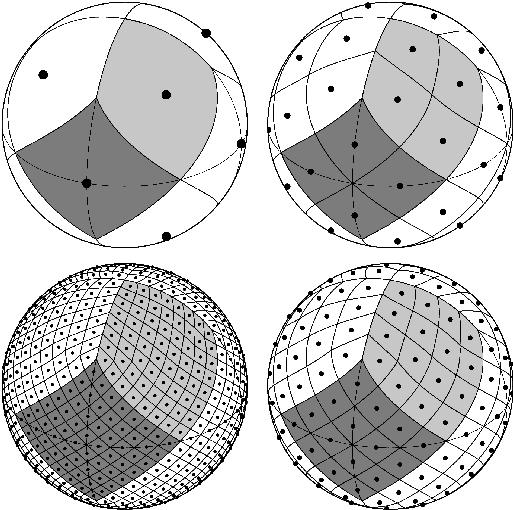
\includegraphics[width=0.5\linewidth]{gorski_f1.jpg}
        \caption{HEALPix tesselation}
        \label{fig:healpix}
    \end{figure}
    \item Uniform sampling
    \item ...
\end{itemize}

\subsection{band-limited signal} %cite soft fourier
 Depending on the sampling density, signal can only be truthfully represented up to lmax spherical harmonic.
 
\section{invariance and equivariance}
what is invariance and equivariance
\begin{equation}
    T_1(f(x)) = f(T_2(x))
\end{equation}
where:
\begin{itemize}
    \item[T] a transformation operation (e.g. a rotation)
    \item[f] a filter
    \item[x] the data analyzed
\end{itemize}
Invariance is when $T_2$ is the identity. Thus the result of the filter will always be the same whichever the transformation. (internal representation is still the same)
same-equivariance is when $T_1 = T_2$, transformation of input is the same transformation of output ans is a special case of equivariance.

classification task are invariant ==> object detection, task invariant, but internal properties are equivariant (being able to tell the orientation, position, lightning, ...) 

why is it useful?

Some signal remains fundamentally the same under a symmetry transformation. Thus, being able to observe the same features through invariance or perceive the transformation through the equivariance, and still see the same data is useful.

in case of cnn, it is for weight sharing. For whatever the transformation is, still see the same object.
Standard CNN very powerful because they are translation equivariant (weight shared for all pixels), thus will react the same if pixels in another location.

In standard CNN, data augmentation is done to learn the equivariance/invariance, or transformation of the input in a space where the desired equivariance can be transformed to a known equivariance (translation in the case of standard CNN. But this equivariance can be (mathematically) encoded directly in the architecture. Meaning that the filters will directly be equivariant and don't need to learn to be it.

(

\section{learning}
%\subsection{CNN}
% Models in deep learning that uses invariance and equivariance are more and more seen
Archictecture that exploits structure and symmetries present in data are powerful because they don't have to learn them and can directly focus on the main features needed for the task. Thus being invariant or equivariant to some symmetry such as translation or rotation in the data domain can speed up the training time, and make the given model more robust to perturbation (translation or rotation).
\subsection{spherical CNNs}
More datasets present rotation symmetries or lie on the sphere $S^2$ (e.g in section \ref{chap:Datasets}). In this section, architectures working on this kind of data are presented, either they are invariant, equivariant or variant to rotations and/or deformation
\subsubsection{2D CNNs on planar projection}
One of the most instinctive use of CNN on spherical data is to use a planar projection of $S^2$. However, there is no perfect unique uniform sampling of the sphere. Some of the different samplings are explained on section \ref{sec:sampling}.

But as there is no perfect uniform sampling, it is not possible to translate the desired equivariance to rotation to an equivariance to translation, because deformation is induced on the projection (see Fig. \ref{fig:planar_projection}). First approaches use standard CNN on equiangular projection. Other projection, such as the cubed sphere\cite{boomsma_spherical_2017}, or platonic solids\cite{cohen_gauge_2019}\cite{jiang_spherical_2019}\cite{lee_spherephd:_2018} may be used to reduce deformation and ..., but may lose the rotation equivariance.

Most models that works on omnidirectional imaging use this method with equiangular projection, and focuse more on a deformation free architecture \cite{su_learning_2017}\cite{ferrari_spherenet:_2018}, and drop the rotation equivariance part, arhuing that it is not necessary, even useful.

\begin{figure}[h!]
    \centering
    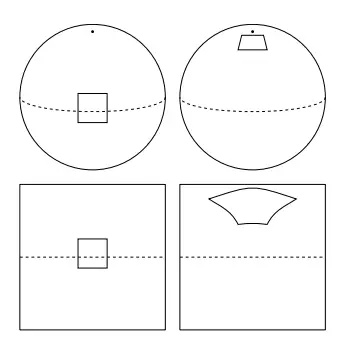
\includegraphics[width=0.5\linewidth]{v2-9d6a9d92bb02bc9e198c4c16397ce2fd_b.jpg}
    \caption{Deformation of planar projection \cite{cohen_spherical_2018}}
    \label{fig:planar_projection}
\end{figure}
% \subsubsection{2D CNNs on pixels}
% * Cohen \cite{cohen_gauge_2019}
% * Jiang \cite{jiang_spherical_2019}
% * ...

gauge transformation. invariance to deformation. iotropic vs anisotropic filters
\subsubsection{SHFT on SO(3) and S2}
One way to reach true equivariance to rotation is to use Spherical Harmonics and go in the spectral domain.
\begin{itemize}
    \item Cohen \cite{cohen_spherical_2018}
    \item Esteves \cite{esteves_learning_2017}
\end{itemize}
Computationnaly expensive as we need to do SHFT every forward pass and backward pass during the training of the neural net.
\subsubsection{Graph CNNs}
Another way to represent the data is to use a graph
* LTS4 \cite{frossard_graph-based_2017}
* DeepSphere \cite{perraudin_deepsphere:_2018}
\begin{figure}[h!]
    \centering
    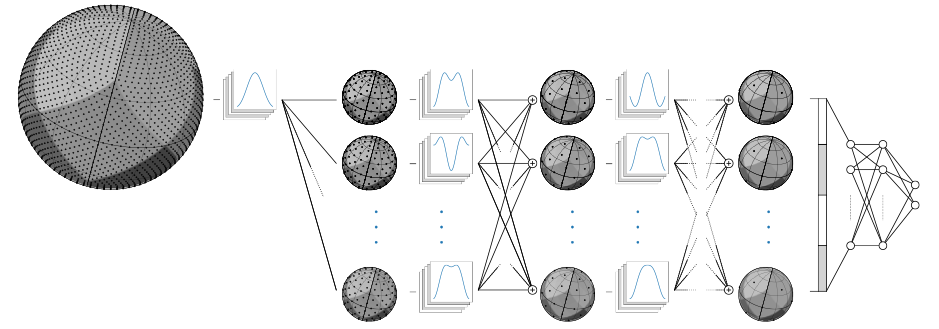
\includegraphics[width=0.8\linewidth]{figure2-Blogpost-SCNN.png}
    \caption{DeepSphere architecture}
    \label{fig:deepsphere}
\end{figure}
* ...

only isotropic filter using monom or polynomial filter (ring hops)

% It is seen that for a spherical graph to keep the rotation equivariance properties, the eigenvectors of its laplacian must approximate the spherical harmonics. Convergence is easily doable if random uniform sampling. %\cite martino
% Possible if as uniform as possible sampling
% equiangular is not one of them

\chapter{Different datasets}\label{chap:Datasets}
\section{3D objects}
Equivariance in rotation useful because the object is the same whatever the orientation is ( an upside down plane is still a plane).

Main problem is that the spherical signal does not represent correctly the 3D object. occlusions are not represented, and only a specific point of view for each vertex is represented.

meilleur representation est graph a partir de vertex. Normalement toujours rotation equivariant, même si approxime plus les harmoniques spheriques.

classifiy only graphs and not signal on graph.

\section{cosmological maps}
see deepsphere paper

need a great resolution to observe features
anisotropic filters is not needed in this case

\section{Omnidirectional imaging}
real life or virtual.
True representation on the sphere (depending on the sensor)

direction of gravity is important
No real rotation symmetry of signal
\subsection{panorama}
Better representation might be the cylinder. In this case, we keep a rotation and the gravity. A plus side is the perfect uniform sampling on the cylinder.
\section{planetarian data}
pseudo spherical data, easily represented by a graph.
But there is no rotation symmetry, or only 1 rotation (spin of the earth)

no similar signal on pole or equator, or on oceans and continents.

but local rotation equivariance may be useful
\subsection{climate on earth}
\subsection{climate aerial}
\subsection{...}
density, economics,...

\section{molecular}

\section{medical imaging}

\section{mocks dataset}
Mainly projection of plane images on the sphere. For example, projection of MNIST digits.

do not represent reality, or real life problem. It is not useful at the end. Only to prove some trivial concepts.

\chapter{Benchmark}

\section{Choice of datasets/tasks}
As the goal of this study is to compare DeepSphere against several spherical CNNs, and prove its advantages, one must chose carefully the datasets. \todo{Pour rappel, }The advantages of Deepshere are its speed and its flexibility. Downsides are only equivariant in $S^2$ by construction and invariant to the third rotation in $SO(3)$, and the almost equivariance due to graph construction.

Need global task, dense task, and a one that prove the flexibility of the model.
\subsection{SHREC17}
shape retrieval task. similar to a global classification task.
This dataset was chosen mainly because it was used to demonstrate the ability of two other spherical CNNs, the models of Cohen and Esteves. there was still room for improvement

train: 31364 instances in 55 classes (non uniform)
val: 633 instances in 55 classes
test: 10265 instances in 55 classes
\subsection{ModelNet40}
real global classification task, used by Esteves and jiang, and compared with Cohen.
train: 9843 instances in 40 class (non uniform)
test: 2468 instances in 40 class

airplane\_0119 cannot support a rotation?

poor population
\subsection{GHCN-daily}
non uniform sampling on the earth with various meteorological information such as temperature, precipitation and snow fall. lots of missing data. will be used as a proof of flexibility of deepsphere model if a task is found.

50469 stations position for every day since 1xxx

\subsection{climate pattern segmentation (ExtremeWeather}
ExtremeWeather dataset from CAM5.1
equirectangular sampling with a 25-km resolution at equator (0.23 deg x 0.31 deg) 
labels are not certain. Task not so useful, but can prove the segmentation on the sphere.
768x1152 pixels = 884'736 px ==> Nside = 256 ==> 786'432 px
Jiang and Cohen used 10*4**5+2 tesselation = 10'242 (bilinear interpolation) ==> Nside = 16 - 32
\subsection{cylinder panoramic}
just an idea
\subsection{just another non uniform dataset}

\section{SHREC17 task}
\subsection{dataset and task}
Task is to develop a 3D shape retrieval method
\begin{figure}[ht]
    \centering
    \includesvg[width=0.5\linewidth]{lamp_000018.svg}
    \caption{Ray-casting on the sphere}
    \label{fig:ray_cast}
\end{figure}
\begin{figure}[ht]
    \centering
    \includesvg[width=0.5\linewidth]{lamp_sphere_000018.svg}
    \caption{Resulting spherical signal}
    \label{fig:sphere_signal}
\end{figure}
\subsection{Cohen Model}
Use an equiangular grid (SOFT) to project the data on the sphere of res x res with res = 2 * bandwidth

\subsubsection{comparison}
Without regularization, our model tend to overfit, and the validation loss increase steadily. But results still seems to become better as the number of epochs become greater (accuracy, f1 score and shrec17 script)

augmentation slightly better result but more stable, robust evolution. Prevent overfitting on the dataset
\subsection{Esteves Model}
Use the same resXres grid as Cohen, but only keep two features

pooling in spectral space
\subsection{Trying to beat them}
As more computationnaly efficient, can do a deeper model.

\subsection{Tweaking our system}
Using an imperfect sampling (equiangular) to be more flexible

Quick analysis of resulting graph
\subsubsection{Construction of equiangular graph}
In order to approximates at best the first spherical harmonics
\subsection{Conclusion}

\subsubsection{Results}
\begin{table}[ht]
    \centering
    \begin{tabular}{l|l l|l l l}
        Method & Accuracy & F1-score & params & sample time & training time \\ \hline
        Cohen\_s2cnn & - & - & 1.4M & 75ms & 50h (245h)\\
        Cohen\_s2cnn\_simple & 78.09 & 78.45 & 400k & 12ms & 32h\\
        Esteves\_sphericalcnn & 79.18 & 79.36 & 500k & 9.8ms & 2h52\\ \hline
        Deepsphere (Cohen-like) & 77.86 & 77.90 & 170k & 17.5ms & 9h43\\
        Deepsphere (Cohen-light) & 76.83 & 76.66 & 60k & 2.8ms & 1h37\\
        %Deepsphere Equiangular & & & & \\
        Deepsphere Best & 80.42 & 80.65 & 190k & 1.6ms & 43m
    \end{tabular}
    \caption{SHREC17 as classification task}
    \label{tab:SHREC17_class}
\end{table}

\begin{table}[ht]
    \centering
    \begin{tabular}{l|c c c c|c c c c}
         & \multicolumn{4}{c|}{micro (label average)} & \multicolumn{4}{c}{macro (instance average)} \\
        Method & P@N & R@N & F1@N & mAP & P@N & R@N & F1@N & mAP \\ \hline
        Furuya\_DLAN & 0.814 & 0.683 & 0.706 & 0.656 & 0.607 & 0.539 & 0.503 & 0.476 \\
        Tatsuma\_ReVGG & 0.705 & 0.769 & 0.719 & 0.696 & 0.424 & 0.563 & 0.434 & 0.418\\ \hline
        Cohen\_s2cnn & 0.701 & 0.711 & 0.699 & 0.676 & - & - & - & - \\
        Cohen\_s2cnn\_simple & 0.699 & 0.693 & 0.690 & 0.657 & 0.473 & 0.522 & 0.476 & 0.426\\
        Esteves\_sphericalcnn & 0.717 & 0.737 & - & 0.685 & 0.450 & 0.550 & - & 0.444\\ \hline
        Deepsphere (Cohen-like) & 0.695 & 0.688 & 0.684 & 0.654 & 0.424 & 0.478 & 0.423 & 0.389\\
        Deepsphere (Cohen-light) & 0.684 & 0.682 & 0.676 & 0.643 & 0.410 & 0.452 & 0.398 & 0.354 \\
        %Deepsphere Equiangular & & & & \\
        Deepsphere Best & 0.725 & 0.717 & 0.715 & 0.686 & 0.475 & 0.508 & 0.468 & 0.428
    \end{tabular}
    \caption{SHREC17 perturbed dataset results}
    \label{tab:SHREC17_retriev}
\end{table}

\todo{IDEA: for a single instance of easy class, and one from undinstiguishable class (flower pot), make several rotation and see evolution of logits and feature map}

\subsection{Misc}
Performance tested on Cohen similar architecture, with 20 epochs and 40 evaluation done on RAM.\\
\begin{tabular}{|c|c|c|c|c|c|}
\hline
~ & Time per batch & CPU time & Wall time & GPU memory & Load average  \\ \hline
\begin{tabular}{c}
Dataset loaded\\
on RAM
\end{tabular}
 & 0.12 s & 1598 s & 2693 s & 1395 MiB & 80\% \\ \hline
\begin{tabular}{c}
Dataset loaded\\
on the fly
\end{tabular}
 & 
\begin{tabular}{c}
0.11 +   \\
0.06 s\\(loading time)
\end{tabular}
& 2541 s & 3667 s & 1395 MiB & 50\% \\ \hline
TF Dataset pipeline & 0.09 s & 2400 s & 2046 s & 1395 MiB & 90\% \\ \hline
\begin{tabular}{c}
TF Dataset\\
pipeline w/ TFRecords
\end{tabular}
 & 
\multicolumn{5}{c|}{TODO in the future to further improve performance} \\ \hline
\end{tabular}

batch time for different parameters:\\
nsides = [32, 64, 128], t = [0.07, 0.26, 1.15] linear in function of number of pixels\\
size of filter (number of hops) K = [5, 4, 2], time = [0.26, 0.19, 0.11] linear in function of number of parameters
\section{Influence of sampling}
\subsection{dataset}
Projection of images, 3D objects on different parts of sphere
Dataset1: projected on equator
Dataset2: project on pole
Dataset3: combination of D1 and D2
Train on D1, D2 and D3 and see how they react on each dataset

Not done, and will maybe not be done. different graph each time. Not change from mock dataset such as Spherical-MNIST
\section{Classification task - ModelNet40}
\subsection{dataset and task}
More or less similar than SHREC17 but with less instances in total

shift 90deg on map give the exact same results, so the implementation is correct.

plant\_0338 is flat and cannot be ray casted.
plant\_0078

problem rotation. not enough sample and indistiguishable.

try with less features (distance and normals, like Esteves). nothing change, same results. confirm that other features can be computed from the first one.

difficult to distinguidh on the sphere signal (for example desk from table)
\subsection{Jiang - Esteves - Cohen models}

\subsection{our result}

\subsection{conclusion}
\section{weather data - GHCN}
\subsection{dataset}
\subsection{find a task}
mask valeur nan
valeur avec interpolation

différent graph?

regression\_tikhonov(G, y, M, tau=0): tau = 0, y = mask

faire 2 graph (min set avec que des bonnes valeurs, super set avec 75\% de valeurs et regression tikhonov

minSet:

test regression temperature future
features: temp for n days, number of day in year, number of month in year
hyperparameters: number of neighbours in NNgraph, number of days, ...
MSE 7.7/10.43 MAE: 2.47, exp\_var: 0.8567, r2: 0.848
remove month as it is redundant with days:
no change, remove later
normalisation of data temperature:
no good
add info about station (position on sphere, altitude)
no good

prédit correctement le jour actuel, et pas le lendemain

hypothèse, need small filter as we don't need to know info on other side planet.
empirical result: better loss and other metrics with high filter and number of neighbours

\section{ExtremeWeather}
\subsection{dataset and task}
\subsection{other models}
\subsection{our model and result}
\subsection{conclusion}

\section{Prove flexibility dataset}
\subsection{dataset and task}
\subsection{our approach}


\chapter{Analysis - Summary}
\chapter{conclusion}
\section{Future Work}
\printbibliography
\addcontentsline{toc}{chapter}{Bibliography}
\appendix
\end{document}